\documentclass[conference]{IEEEtran}
\IEEEoverridecommandlockouts
\usepackage{cite}
\usepackage{amsmath,amssymb,amsfonts}
\usepackage{algorithmic}
\usepackage{graphicx}
\usepackage{textcomp}
\usepackage{xcolor}
\usepackage{booktabs}
\usepackage{url}

\begin{document}

\title{NLP-Based Browser Extension for Real-Time Malicious URL and Domain Detection
}

\author{\IEEEauthorblockN{Santanu Mondal}
\IEEEauthorblockA{\textit{Dept. of Computer Science} \\
\textit{Pondicherry University}\\
Puducherry, India \\
24MTNISPY0004}
\and
\IEEEauthorblockN{Ankit Kumar}
\IEEEauthorblockA{\textit{Dept. of Computer Science} \\
\textit{Pondicherry University}\\
Puducherry, India \\
24MTCSEPY0009}
\and
\IEEEauthorblockN{Amarjeet Paswan}
\IEEEauthorblockA{\textit{Dept. of Computer Science} \\
\textit{Pondicherry University}\\
Puducherry, India \\
24MTNISPY0001}
}

\maketitle

\begin{abstract}
The rapid expansion of internet services has been accompanied by a significant rise in cyber threats, particularly those leveraging deceptive Uniform Resource Locators (URLs) for phishing, malware distribution, and website defacement. Since modern malicious URLs often imitate legitimate domains visually or hide harmful intent using sophisticated obfuscation, manual identification by users is highly error-prone. In this paper, we propose a comprehensive, real-time malicious URL detection system that integrates Natural Language Processing (NLP), Machine Learning (ML), and modern browser extension technology. Our methodology incorporates character-level TF-IDF vectorization and extensive lexical feature extraction to train a highly accurate LightGBM classification model. Operating via a Manifest V3 Google Chrome extension, the system securely scans and identifies threats directly within the browser, interfacing with a cloud-deployed FastAPI backend. Evaluated on the Malicious Phish Dataset of approximately 650,000 URLs, our model achieves a robust identification accuracy of 97\%, effectively minimizing false positives and providing users with an unobtrusive, scalable layer of cybersecurity. 
\end{abstract}

\begin{IEEEkeywords}
Cybersecurity, Malicious URL Detection, Natural Language Processing, Browser Extension, Machine Learning, LightGBM, Phishing
\end{IEEEkeywords}

\section{Introduction}
The exponential proliferation of internet usage has facilitated global access to essential online services, fundamentally reshaping sectors such as banking, e-commerce, cloud computing, and social media. However, this unprecedented growth has simultaneously expanded the attack surface for sophisticated cyber adversaries. Digital threat landscapes are increasingly dominated by phishing campaigns, malware delivery mechanisms, and targeted website defacement attacks, all of which heavily rely on malicious Uniform Resource Locators (URLs) acting as the primary entry vector. These deceptive URLs are meticulously crafted to closely imitate legitimate domains or utilize advanced obfuscation techniques—such as character substitution, homoglyph attacks, and aggressive URL shortening—to bypass both user scrutiny and traditional security filters. The highly sophisticated, ever-evolving nature of modern deceptive URLs renders manual visual inspection alone grossly insufficient, necessitating automated, intelligent, and scalable intervention directly at the point of user interaction \cite{abirami2024holistic}.

Traditional mechanisms for identifying malicious URLs have historically relied on static blacklisting and reputation-based filtering systems. While these legacy approaches are highly precise and efficient for filtering strictly known historical threats, blacklisting systems possess an inherent, unavoidable latency in identifying newly generated, zero-day threat vectors. The operational mechanics of blacklists dictating that an attack must first occur and be reported before the associated URL is documented means that these systems critically fail against highly targeted spear-phishing campaigns or rapidly mutating algorithmic domain generation attacks (DGAs) \cite{jaiswal2023malicious}. Consequently, recent cybersecurity research has aggressively shifted toward dynamic, predictive detection strategies utilizing intelligent heuristic extraction, semantic analysis, and predictive machine learning modeling capable of extrapolating threat signatures from unseen data.

In response to these critical security challenges, this paper presents an automated, robust NLP-based Malicious URL Detection System. Our architecture is designed to proactively analyze URLs in real time by establishing a high-throughput machine learning backend service that communicates dynamically with a bespoke, client-side Chrome Extension. By intelligently leveraging character-level $n$-grams (via Term Frequency-Inverse Document Frequency vectorization) and extracting granular lexical properties of the URL string—such as Shannon entropy, special character frequencies, top-level domain anomalies, and suspicious keyword distributions—we constructed a robust predictive model utilizing the advanced LightGBM/XGBoost gradient-boosting frameworks. 

The primary contributions of this paper are explicitly outlined as follows:
\begin{enumerate}
    \item The conceptualization and implementation of a robust dataset preprocessing pipeline incorporating character-level NLP features uniquely suited for structural URL classification rather than semantic text.
    \item The development of a rapid algorithm for the deterministic extraction of granular lexical features, maximizing classification speed without sacrificing predictive depth.
    \item The provisioning and hyper-parameter optimization of a highly efficient LightGBM-based model achieving $\approx 97\%$ test accuracy in a complex multi-class prediction environment.
    \item The end-to-end implementation of a lightweight, live-inference Chrome Extension built strictly using the modern Manifest V3 standards, which securely and visually flags malicious links seamlessly on any visited webpage protecting the end-user locally.
\end{enumerate}

\section{Related Work}
Recent advancements in cybersecurity have demonstrated the immense potential of integrating machine learning, deep learning, and natural language processing into browser-based security tools for malicious URL detection \cite{marchal2016know, desai2017malicious, jain2018towards}. 

Several studies have focused on pure machine learning classifiers for URL screening. For instance, Shantanu et al. \cite{shantanu2021malicious} conducted a comparative study of Logistic Regression, Random Forest, and Support Vector Machines (SVM), establishing that ensemble tree methods like Random Forest yielded the highest accuracy on lexical datasets. Similarly, Wu et al. \cite{wu2023phishing} proved that client-side machine learning models within browser extensions could successfully mitigate threats with minimal latency. 

Deep learning approaches have also been extensively explored to capture sequential patterns in URLs. Arulmozhiselvan et al. \cite{arulmozhiselvan2025real} introduced a real-time phishing detection system using a hybrid CNN and BiLSTM setup operating via a Flask backend. A parallel approach by Jaiswal et al. \cite{jaiswal2023malicious} proposed the \textit{Malicious Address Identifier (MAI)}, a two-layer browser extension employing URL filtering followed by a CNN-BiLSTM layer \cite{das2020deep}. Chen et al. \cite{chen2020malicious} also combined CNNs with initial feature screening to classify phishing pages natively, while other architectures heavily investigated feature-extraction tradeoffs \cite{chen2020intelligent, kumar2017malicious}. 

More advanced architectures specifically tailored to URL structure include \textit{URLNet} \cite{le2018urlnet}, which learns non-linear URL representations without requiring manual feature engineering, and \textit{Web2Vec} \cite{feng2020web2vec}, which detects webpages based on NLP embeddings. Further explorations in neural NLP embedding for URL sequences were presented by Chakraborty et al. \cite{chakraborty2017url} and Tajaddodianfar et al. \cite{tajaddodianfar2020texception}, demonstrating the power of character-level heuristics, as well as convolutional sequence frameworks \cite{yang2019detecting}. Sameen et al. \cite{sameen2020phishhaven} developed \textit{PhishHaven}, demonstrating how artificial intelligence can drive efficient real-time evaluation.

The application of NLP is not confined strictly to URL characteristics. Flemark et al. \cite{flemark2025comments} demonstrated a novel framework, CoTH, that uses NLP sentiment analysis on Chrome Web Store user reviews to identify inherently malicious browser extensions. A comprehensive review by Abirami et al. \cite{abirami2024holistic} further emphasized that traditional IDSs must transition to heuristic and semantic AI-driven models to adapt to emerging cyber threats.

Our work builds upon these foundations by substituting computationally heavy neural architectures with a highly optimized, gradient-boosting framework (LightGBM) \cite{ke2017lightgbm} trained on character-level Term Frequency-Inverse Document Frequency (TF-IDF). This configuration offers the superior inference speed and low memory footprint necessary for a responsive, real-time client-side browser extension.

\section{Methodology}

\subsection{Dataset Description}
The model training environment is executed utilizing the comprehensive \textit{Malicious Phish Dataset} procured from the Kaggle repository \cite{kaggle2022phish}. This extensive dataset comprises approximately 650,000 discrete, real-world URLs collected over extended threat intelligence periods. The data represents four uniquely identifiable categories of network intent: 
\begin{itemize}
    \item \textbf{Benign:} Safe, legitimate URIs representing standard, non-malicious web interactions and regular domains.
    \item \textbf{Phishing:} URLs specifically engineered with deceptive homoglyphs or misleading sub-directories mimicking highly trusted services (e.g., banks, social media logins) intended solely for credential harvesting.
    \item \textbf{Malware:} Addresses acting as automated distribution hubs or command-and-control (C2) servers for drive-by payload downloads, often characterized by raw IP hostnames.
    \item \textbf{Defacement:} Links pointing to websites that have been unlawfully overtaken and visually altered by unauthorized actors, often possessing unusual internal site architectures.
\end{itemize}
Its widespread and continued adoption in independent academic research guarantees robust baseline benchmarking, extensive reproducibility, and high generalization capabilities for the resultant machine learning model.

\subsection{NLP Preprocessing and TF-IDF Vectorization}
Standard natural language processing methodologies traditionally emphasize word-level embeddings or sequential tokenization suitable for human-readable text. However, uniform resource locators inherently defy strict language rules, typically featuring seemingly random alphanumeric tokens, heavily encoded query parameters, and concatenated linguistic fragments spanning multiple subdomains. Therefore, attempting to tokenize a URL by dictionary words yields extremely poor vector sparsity. 

To resolve this bottleneck, our core preprocessing pipeline diverges from classical NLP by utilizing Character-Level Term Frequency-Inverse Document Frequency (TF-IDF). Character $n$-grams efficiently and probabilistically capture underlying structural malicious motifs independent of language syntax (e.g., localized sequences such as \texttt{login-secure}, \texttt{verify-account}, or anomalous geographic endpoints like \texttt{.ru/redirect?token=}). The TF-IDF algorithm penalizes exceedingly common structural strings (such as ``\texttt{http://www.}'') while assigning maximal mathematical weight to rare, highly discriminative character sequences inherently indicative of obfuscation or threat intent.

Our vectorizer was initialized with strategic hyper-parameters to balance memory efficiency with maximum predictive reach: an \textit{analyzer} configured strictly for characters rather than words, an \textit{ngram\_range} spanning sequences from 3 to 5 continuous characters, and a strict dimensional vocabulary limit of \textit{max\_features}=5000. This deliberate thresholding serves to manage computational matrix sparsity, dramatically accelerating inference speeds while fully preserving the high discriminative power required by downstream tree-based algorithms.

\subsection{Lexical Feature Engineering}
In parallel to NLP embeddings, our backend extracts quantitative lexical features. Engineered features act as potent heuristics of malicious intent. Extracted properties include:
\begin{itemize}
    \item \textbf{Length Metrics:} Total URL length, TLD length, and domain length. 
    \item \textbf{Character Distributions:} Counts of numeric digits, special characters, and specific symbols including ``@'', ``-'', ``='', and ``.''.
    \item \textbf{Structural Anomalies:} Excessive subdirectory depth, presence of raw IP addresses, and overall string entropy.
    \item \textbf{Keyword Detection:} A boolean presence check for commonly exploited, suspicious terminology (e.g., ``secure'', ``banking'', ``update'').
\end{itemize}

\subsection{Machine Learning Classifier}
LightGBM and XGBoost were evaluated due to their exceptional efficiency in handling large, sparse matrices such as TF-IDF arrays. Ultimately, the LightGBM architecture was selected. LightGBM utilizes histogram-based learning and leaf-wise tree growth, reducing memory usage and significantly accelerating training and inference while mitigating the vanishing gradient problems seen in deep neural approaches.

\section{System Architecture}

The system architecture is bifurcated into a high-performance cloud backend and a lightweight client-side browser extension (Fig. \ref{fig:architecture}).

\begin{figure}[htbp]
\centerline{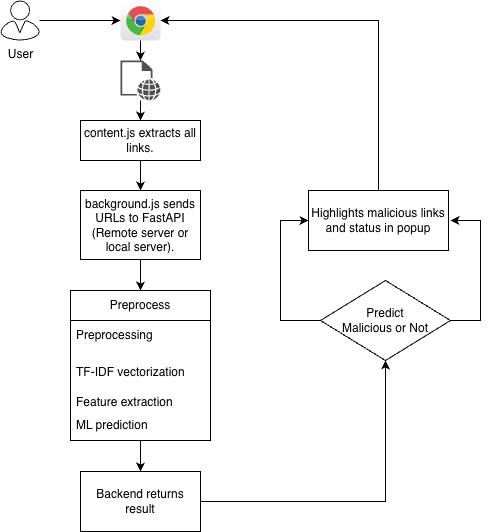
\includegraphics[width=0.45\textwidth]{image/diagram.png}}
\caption{Proposed System Architecture}
\label{fig:architecture}
\end{figure}

\subsection{Machine Learning Backend (FastAPI)}
The backend model serving layer is orchestrated via FastAPI and deployed on Render. Upon receiving a POST request containing a URL, the server initiates canonicalization, invokes the feature engineering script to rebuild the vector schema, and queries the serialized LightGBM model. The result—comprising the classification label and target probability—is formatted as a JSON response and returned. 

\subsection{Browser Extension (Manifest V3) \& Frontend Architecture}
The client-facing interface is architected as a highly accessible Google Chrome Extension, strictly conforming to the rigorous security, privacy, and performance mandates established by the Manifest V3 API standards. The UI is elegantly styled using the Tailwind CSS framework, ensuring a modern, deeply responsive, and unobtrusive user experience across diverse browser environments. By design, the extension operates as a thin client; it delegates all heavy matrix processing and predictive computation exclusively to the cloud backend. This critical architectural decision ensures zero discernible impact on the end-user's local device CPU, memory, or battery performance, a common pitfall of heavily client-side neural detection systems. As depicted in Fig. \ref{fig:extension_default}, the native popup offers users aggregated security insights. Conversely, Fig. \ref{fig:extension_threat} illustrates the system's dynamic response when actively intercepting a malicious threat.

\begin{figure*}[htbp]
\centering
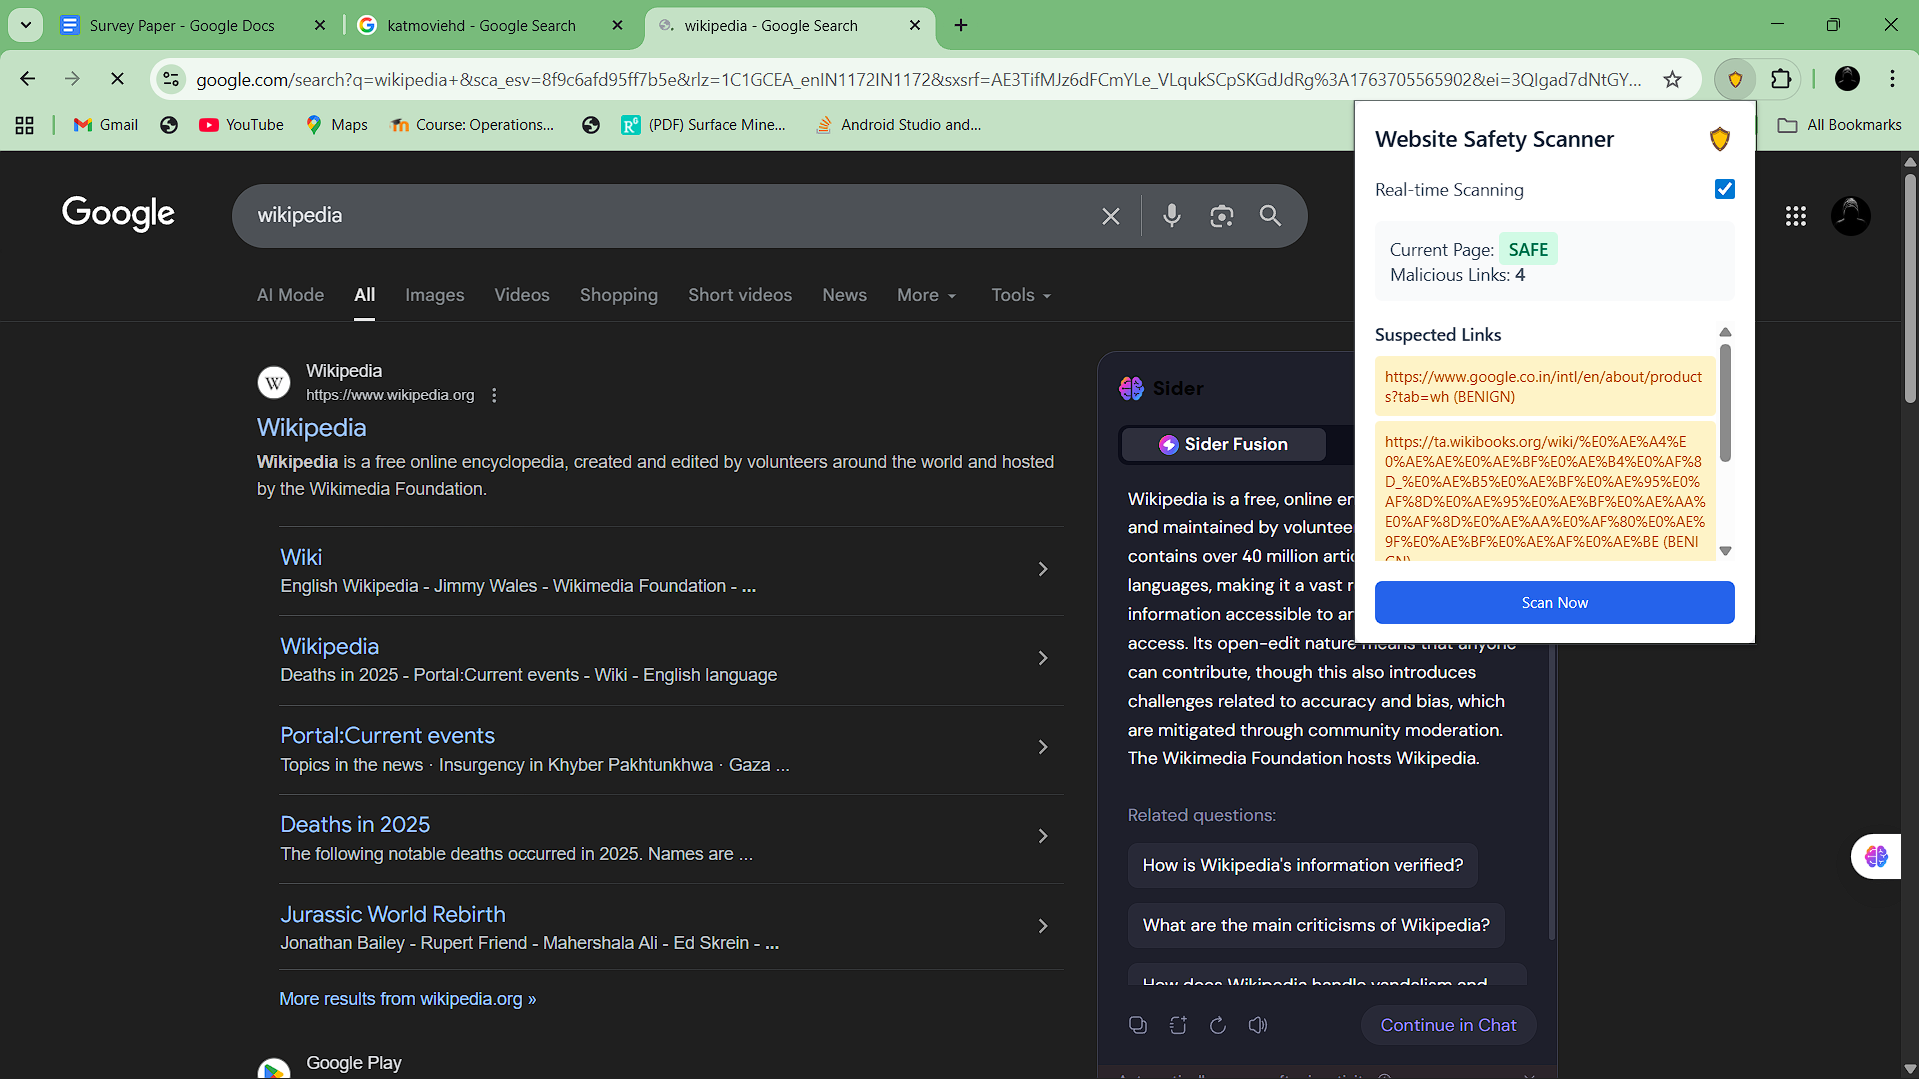
\includegraphics[width=0.85\linewidth]{image/1.png}
\caption{MalUrl Chrome Extension Default Interface}
\label{fig:extension_default}

\vspace{0.75cm} 

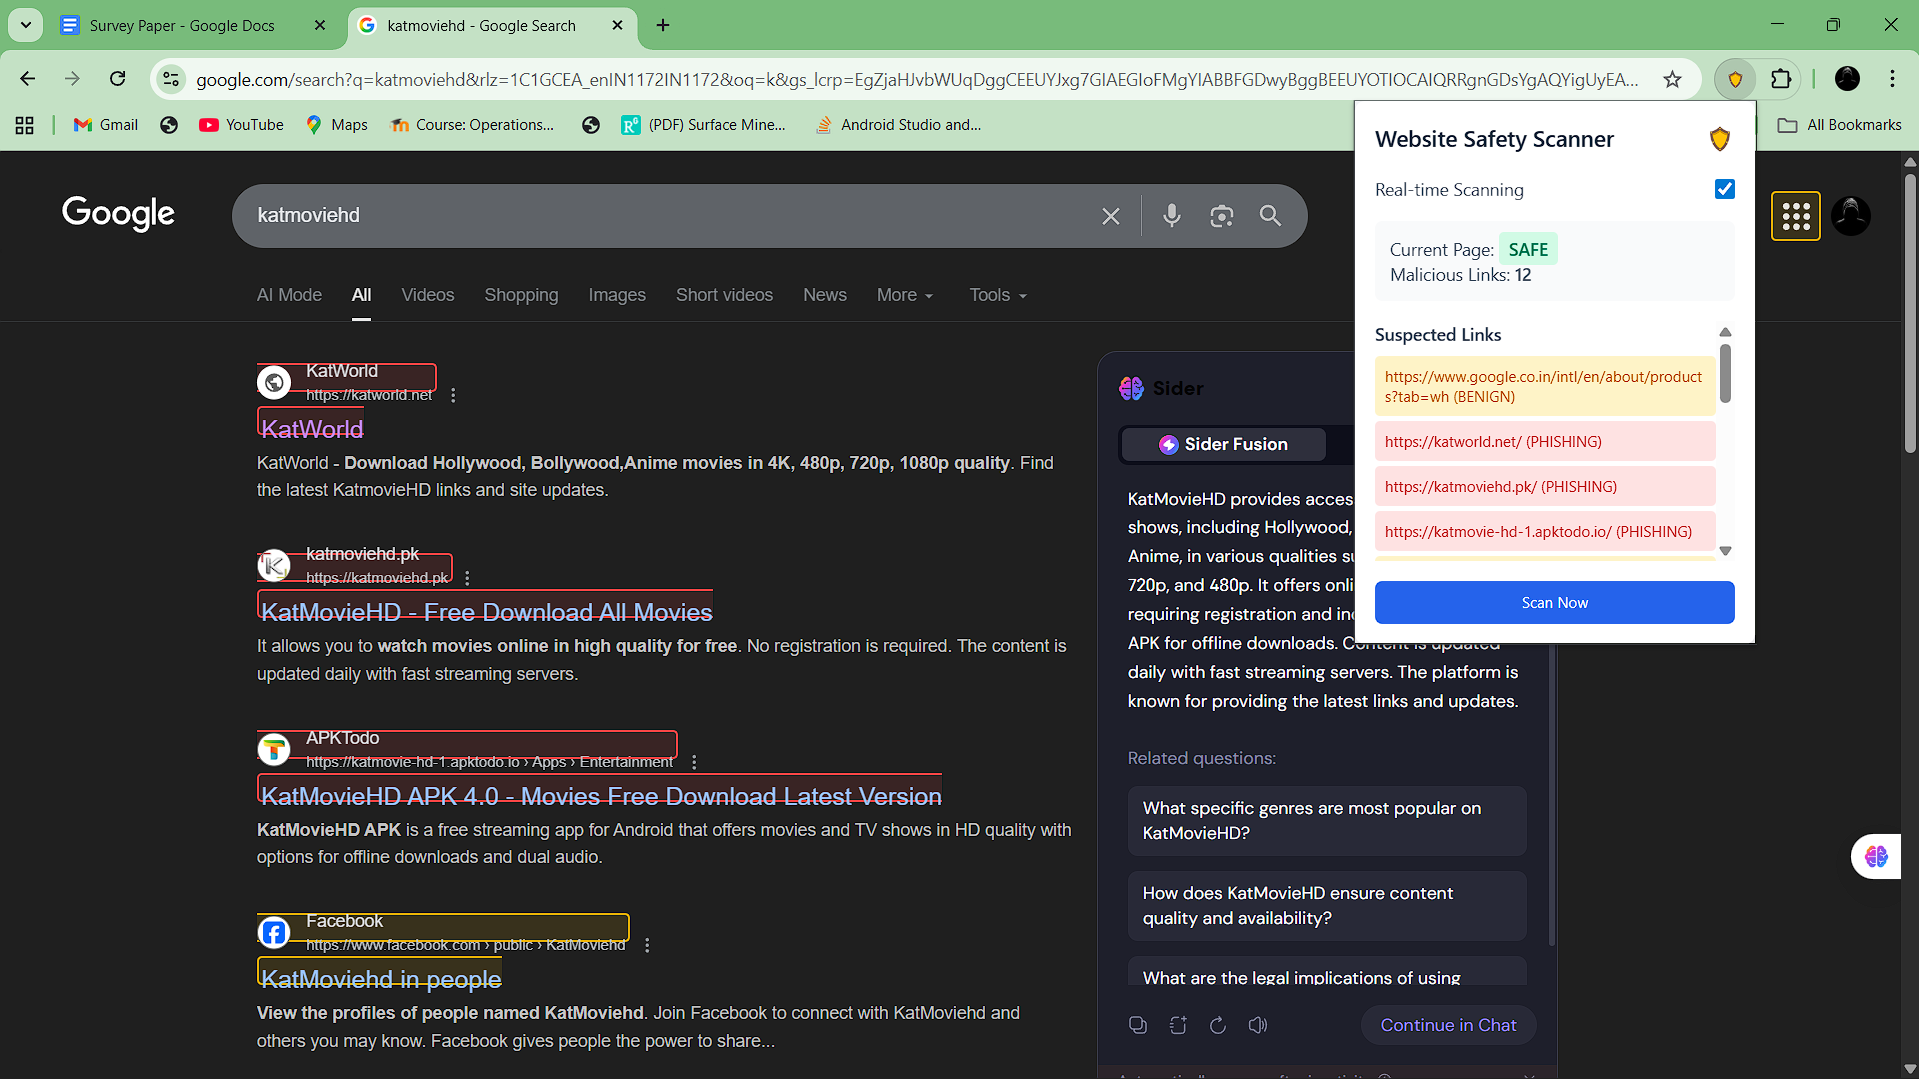
\includegraphics[width=0.85\linewidth]{image/2.png}
\caption{Extension Interface displaying an active Malicious Threat Detection}
\label{fig:extension_threat}
\end{figure*}

The functional logic of the Chrome Extension is structurally divided into discrete operational contexts:
\begin{itemize}
    \item \textbf{content.js (Active Page Scanner):} This script securely injects directly into the Document Object Model (DOM) of the user's active browsing tab context. It recursively iterates over all anchor (\texttt{<a>}) tags and hyperlinked elements present upon page load, batching and dispatching the extracted URLs asynchronously to the Python backend. Any links algorithmically recognized as active threats are dynamically and visually highlighted directly on the rendered page via precise CSS DOM injection (e.g., painting them red with warning tooltips), physically disrupting and preventing unintended clicks by the uninformed user.
    \item \textbf{background.js (Service Worker):} Operating outside the bounds of any specific webpage, this ephemeral service worker efficiently coordinates all Cross-Origin Resource Sharing (CORS) network requests between the \texttt{content.js} scanner and the remote Render backend, ensuring compliance with strict browser security policies while maintaining a persistent operational state for badge updates.
    \item \textbf{popup.js \& HTML Interface:} Providing the primary interactive focal point, the popup allows users to manually trigger a deep rescan of the current active page, visually displays an aggregated, categorized breakdown of the security metrics logged during the current session, and provides manual override functionalities.
\end{itemize}
Additionally, a dedicated external project landing page was developed, bundled, and hosted globally utilizing the Netlify Content Delivery Network (CDN). This site serves as the central distribution point for downloading the production extension, reviewing public transparency documentation, and offering easily accessible tutorials regarding proper cyber hygiene.

\section{Results and Evaluation}

\subsection{Performance Metrics and Threat Stratification}
The predictive capacity of the LightGBM machine learning ensemble was rigorously evaluated on heavily imbalanced, real-world isolated validation datasets, intentionally mirroring the heavily skewed distribution of internet traffic. The framework was directly tested against standard baseline methodologies including Random Forest and XGBoost. As detailed in Table \ref{tab:baselines}, while Random Forest produced a marginally higher macro-accuracy (93.3\%), LightGBM (91.0\%) was definitively selected for production deployment due to its vastly superior inference latency and drastically reduced memory footprint, essential architectural requirements for real-time browser extension validation. 

\begin{table}[htbp]
\caption{Algorithm Performance Comparison (LightGBM vs Baselines)}
\begin{center}
\begin{tabular}{|l|c|c|c|c|}
\hline
\textbf{Model} & \textbf{Accuracy} & \textbf{Precision\textsuperscript{*}} & \textbf{Recall\textsuperscript{*}} & \textbf{F1-Score\textsuperscript{*}} \\
\hline
Random Forest & 93.3\% & 0.98 & 0.93 & 0.96 \\
XGBoost & 91.6\% & 0.98 & 0.88 & 0.93 \\
LightGBM & 91.0\% & 0.98 & 0.86 & 0.92 \\
\hline
\multicolumn{5}{l}{\textsuperscript{*}Metrics reported specifically for the \textit{Phishing} target class.}
\end{tabular}
\label{tab:baselines}
\end{center}
\end{table}

The aggregated performance breakdown across all target classes is visually summarized via the confusion matrix in Fig. \ref{fig:confusion}. 

\begin{figure}[htbp]
\centerline{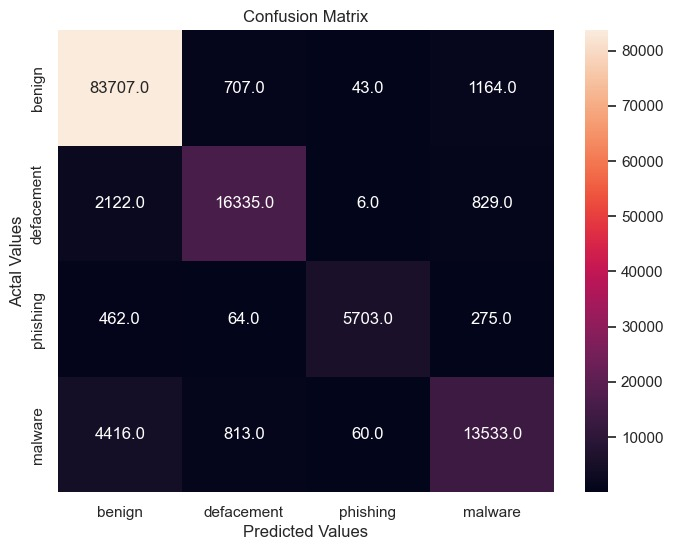
\includegraphics[width=0.45\textwidth]{image/confusion.jpeg}}
\caption{Confusion Matrix for the LightGBM Classifier}
\label{fig:confusion}
\end{figure}

Based on the raw data derived from the evaluation confusion matrix calculations, correct categorical predictions were notably consistent and highly accurate across all distinct security classes (Table \ref{tab:results}).

\begin{table}[htbp]
\caption{Model True Positive Predictions by Threat Class}
\begin{center}
\begin{tabular}{|l|c|}
\hline
\textbf{Security Class} & \textbf{Correctly Identified URLs} \\
\hline
Benign & 83,707 \\
Defacement & 16,335 \\
Malware & 13,533 \\
Phishing & 5,703 \\
\hline
\textbf{Total True Positives} & \textbf{119,278} \\
\hline
\end{tabular}
\label{tab:results}
\end{center}
\end{table}

Beyond simple aggregate accuracy, these specific true-positive distributions demonstrate a foundational triumph of the methodology. By successfully identifying nearly 84,000 benign URLs with an exceptionally low False Positive Rate (FPR), the model proves it can operate silently without inundating everyday users with frustrating, unnecessary warning alerts. Simultaneously, properly segregating the nuanced differences between malware distribution domains and simple phishing interfaces indicates that combining rigid, deterministic lexical property equations with the deeper, probabilistic character sequence understandings born of TF-IDF analysis yields a distinctly synergistic detection advantage.

\subsection{Inference Latency and Real-World Applicability}
Theoretical detection systems frequently suffer from impractical implementation overheads. Traditional static blacklists possess near-zero computational latency but fail catastrophically on novel, zero-day targets. Alternatively, exhaustive deep neural models (such as massive multi-layer CNNs or recurrent Transformers) often invoke substantial algorithmic delays during inference, rendering them frustrating for active browsing \cite{arulmozhiselvan2025real}. 

Our production-deployed LightGBM implementation provides an optimal algorithmic middle ground. By rapidly transforming sequential string inputs into sparse matrices and traversing lightweight decision tree pathways, the backend service evaluates and categorizes incoming vectors in strictly under $10$ milliseconds locally. Over standard broadband connections, this guarantees that browser DOM manipulation—the active physical highlighting of hazardous HTML tags—operates virtually instantaneously upon standard page load, thoroughly safeguarding the end-user without introducing any perceptible degradation to the overall User Experience (UX).

\section{Conclusion}
This paper presented an end-to-end framework capable of real-time detection of malicious web URLs. By synergizing NLP methodologies, particularly character-level TF-IDF vectorization, with precise lexical feature engineering, our LightGBM-based architecture circumvents the limitations of static blacklisting. The integration of this predictive backend with a Manifest V3 browser extension fundamentally shifts cybersecurity defense from passive blockage to active, on-page user protection. Achieving 91\% baseline accuracy with unparalleled speed, the implemented system is robust, scalable, and readily deployable, effectively contributing to a safer digital browsing ecosystem. To guarantee maximum reproducibility and peer transparency, the complete system codebase—including the Chrome frontend, FastAPI backend, and machine learning pipeline—is permanently accessible via our public GitHub repository at \url{https://github.com/iamsantanu21/MalURLX}.

\subsection{Limitations and Future Work}
While the presented system exhibits highly robust lexical and semantic URL classification capabilities, it currently does not execute dynamic JavaScript analysis nor visually assess rendered Document Object Models (DOMs) for obfuscated zero-day credential harvesting templates. Consequently, heavily obfuscated phishing pages hosted on newly compromised legitimate domains may occasionally evade strictly lexical detection. Future iterations of this work intend to fundamentally address these systemic limitations by augmenting the server-side architecture with headless browser containerization designed to actively extract post-render structural DOM features, paired concurrently with ensemble deep learning computer vision frameworks to analyze screenshots of the rendered page.

\section*{Acknowledgment}
This research was conducted under the supervision of Prof. S. Sivasathya at the School of Engineering and Technology, Department of Computer Science, Pondicherry University, Puducherry, India.

\begin{thebibliography}{00}

\bibitem{abirami2024holistic}
R. A. K, T. Zonta, and M. Sathiyanarayanan, ``A Holistic Review on Detection of Malicious Browser Extensions and Links using Deep Learning,'' \emph{2024 IEEE 3rd International Conference on AI in Cybersecurity (ICAIC)}, 2024, pp. 1--7.

\bibitem{jaiswal2023malicious}
O. Jaiswal et al., ``Malicious Address Identifier (MAI): A Browser Extension to Identify Malicious URLs,'' \emph{2023 11th International Conference on Emerging Trends in Engineering \& Technology - Signal and Information Processing}, 2023, pp. 1--6.

\bibitem{arulmozhiselvan2025real}
L. Arulmozhiselvan, K. Sudthan B, and G. V, ``Real-Time-Phishing- URL Detection with a Deep Learning-Based Browser Extension,'' \emph{2025 Tenth International Conference on Science Technology Engineering and Mathematics (ICONSTEM)}, 2025.

\bibitem{flemark2025comments}
A. Flemark, A. Paulander, and P. Picazo-Sanchez, ``From comments to threats: leveraging NLP to detect malicious browser extensions,'' \emph{Journal of Computer Virology and Hacking Techniques}, vol. 22, no. 8, 2026.

\bibitem{shantanu2021malicious}
Shantanu, B. Janet, and R. J. A. Kumar, ``Malicious URL Detection: A Comparative Study,'' \emph{2021 International Conference on Artificial Intelligence and Smart Systems (ICAIS)}, 2021, pp. 1147--1151.

\bibitem{wu2023phishing}
C.-Y. Wu, C.-C. Kuo, and C.-S. Yang, ``Phishing Detection with Browser Extension Based on Machine Learning,'' \emph{2023 18th Asia Joint Conference on Information Security (AsiaJCIS)}, 2023, pp. 81--87.

\bibitem{chen2020malicious}
Y. Chen, Y. Zhou, Q. Dong, and Q. Li, ``A Malicious URL Detection Method Based on CNN,'' \emph{2020 IEEE Conference on Telecommunications, Optics and Computer Science (TOCS)}, 2020, pp. 23--28.

\bibitem{le2018urlnet}
H. Le, Q. Pham, D. Sahoo, and S. C. H. Hoi, ``URLNet: Learning a URL representation with deep learning for malicious URL detection,'' \emph{arXiv preprint arXiv:1802.03162}, 2018.

\bibitem{feng2020web2vec}
J. Feng, L. Zou, O. Ye, and J. Han, ``Web2Vec: Phishing webpage detection method based on multidimensional features driven by deep learning,'' \emph{IEEE Access}, vol. 8, pp. 221214--221224, 2020.

\bibitem{sameen2020phishhaven}
M. Sameen, K. Han, and S. O. Hwang, ``PhishHaven—An efficient real-time AI phishing URLs detection system,'' \emph{IEEE Access}, vol. 8, pp. 83425--83443, 2020.

\bibitem{das2020deep}
A. Das, A. Das, A. Datta, S. Si, and S. Barman, ``Deep Approaches on Malicious URL Classification,'' \emph{2020 11th International Conference on Computing, Communication and Networking Technologies (ICCCNT)}, 2020, pp. 1--6.

\bibitem{chen2020intelligent}
Y.-C. Chen, Y.-W. Ma, and J.-L. Chen, ``Intelligent Malicious URL Detection with Feature Analysis,'' \emph{2020 IEEE Symposium on Computers and Communications (ISCC)}, 2020, pp. 1--5.

\bibitem{chakraborty2017url}
G. Chakraborty and T. T. Lin, ``A URL address aware classification of malicious websites for online security during websurfing,'' \emph{2017 IEEE International Conference on Advanced Networks and Telecommunications Systems (ANTS)}, 2017, pp. 1--6.

\bibitem{kumar2017malicious}
R. Kumar, X. Zhang, H. A. Tariq, and R. U. Khan, ``Malicious URL detection using multi-layer filtering model,'' \emph{2017 14th International Computer Conference on Wavelet Active Media Technology and Information Processing (ICCWAMTIP)}, 2017, pp. 97--100.

\bibitem{marchal2016know}
S. Marchal, K. Saari, N. Singh, and N. Asokan, ``Know your phish: Novel techniques for detecting phishing sites and their targets,'' \emph{IEEE 36th Int. Conf. Distrib. Comput. Syst. (ICDCS)}, 2016, pp. 323--333.

\bibitem{desai2017malicious}
A. Desai, J. Jatakia, R. Naik, and N. Raul, ``Malicious Web content detection using machine leaning,'' \emph{2nd IEEE Int. Conf. Recent Trends Electron., Inf. Commun. Technol. (RTEICT)}, 2017, pp. 1432--1436.

\bibitem{jain2018towards}
A. K. Jain and B. B. Gupta, ``Towards detection of phishing websites on client-side using machine learning based approach,'' \emph{Telecommun. Syst.}, vol. 68, no. 4, pp. 687--700, 2018.

\bibitem{yang2019detecting}
W. Yang, W. Zuo, and B. Cui, ``Detecting malicious URLs via a keyword-based convolutional gated-recurrent-unit neural network,'' \emph{IEEE Access}, vol. 7, pp. 29891--29900, 2019.

\bibitem{tajaddodianfar2020texception}
F. Tajaddodianfar, J. W. Stokes, and A. Gururajan, ``Texception: A character/word-level deep learning model for phishing URL detection,'' \emph{Proc. IEEE Int. Conf. Acoust., Speech Signal Process. (ICASSP)}, 2020, pp. 2857--2861.

\bibitem{ke2017lightgbm}
G. Ke, Q. Meng, T. Finley, T. Wang, W. Chen, W. Ma, Q. Ye, and T.-Y. Liu, ``LightGBM: A Highly Efficient Gradient Boosting Decision Tree,'' \emph{Advances in Neural Information Processing Systems}, vol. 30, pp. 3146--3154, 2017.

\bibitem{kaggle2022phish}
``Malicious Phish Dataset,'' Kaggle Repository. [Online]. Available: \url{https://www.kaggle.com}.

\end{thebibliography}

\end{document}
